\documentclass[]{IEEEtran}
% some very useful LaTeX packages include:
%\usepackage{cite}      
\usepackage{graphicx}   
\usepackage{subfigure} 
\usepackage{url}       
\usepackage{amsmath}    
\usepackage{caption2}
% Your document starts here!
\begin{document}

% Define document title and author
	\title{Weekly Report}
	\author{Adviser: Prof. Yang Wen \\Student: Cheng Wensheng\\ Period: 2018.8.12-8.19
	}
	\markboth{Visual Information Processing Group}{}
	\maketitle

% Write abstract here
\begin{abstract}
	This week I mainly put my effort on improving deep learning methods accuracy of building extraction in SAR images.
\end{abstract}

% Each section begins with a \section{title} command
\section{Sar contest}
	% \PARstart{}{} creates a tall first letter for this first paragraph
	\PARstart{I}{n} this contest, we have tried both deep learning and traditional methods. From the results, we can see that deep learning methods behave better than traditional methods. So we turn to deep learning methods this week.	
	\begin{itemize}
		\item As suggested by Prof.Yang, we decided to try data augmentation techniques, including random crop, flipping and rotation methods.
		\item To improve the number of training samples, I adopted random crop. The result shows that it has improved by 2$\%$. The website also shows 59$\%$ F1 score.
		\item Then I tried flipping and rotation methods, but the result didn't exceed the original ones. I even used pix2pix GAN network, but it behaves worse than original ones.
		\item We need to adjust the deep CNN and use some post-process methods to refine the results.
	\end{itemize}
	
	Fig.~\ref{fig:fw} is the deep learning methods result. Fig.~\ref{fig:rt} is the ground truth image.
	

% Main Part

\newpage
\begin{figure}[!hbt]
%		 Center the figure.
		\vspace{0.7cm}
%		\hspace{50cm}
		\begin{center}
			
\includegraphics[width=0.7\columnwidth]{fw}
				%		 Create a subtitle for the figure.
			\caption{CNN methods result}
			\label{fig:fw}
		    \vspace{0.2cm}
			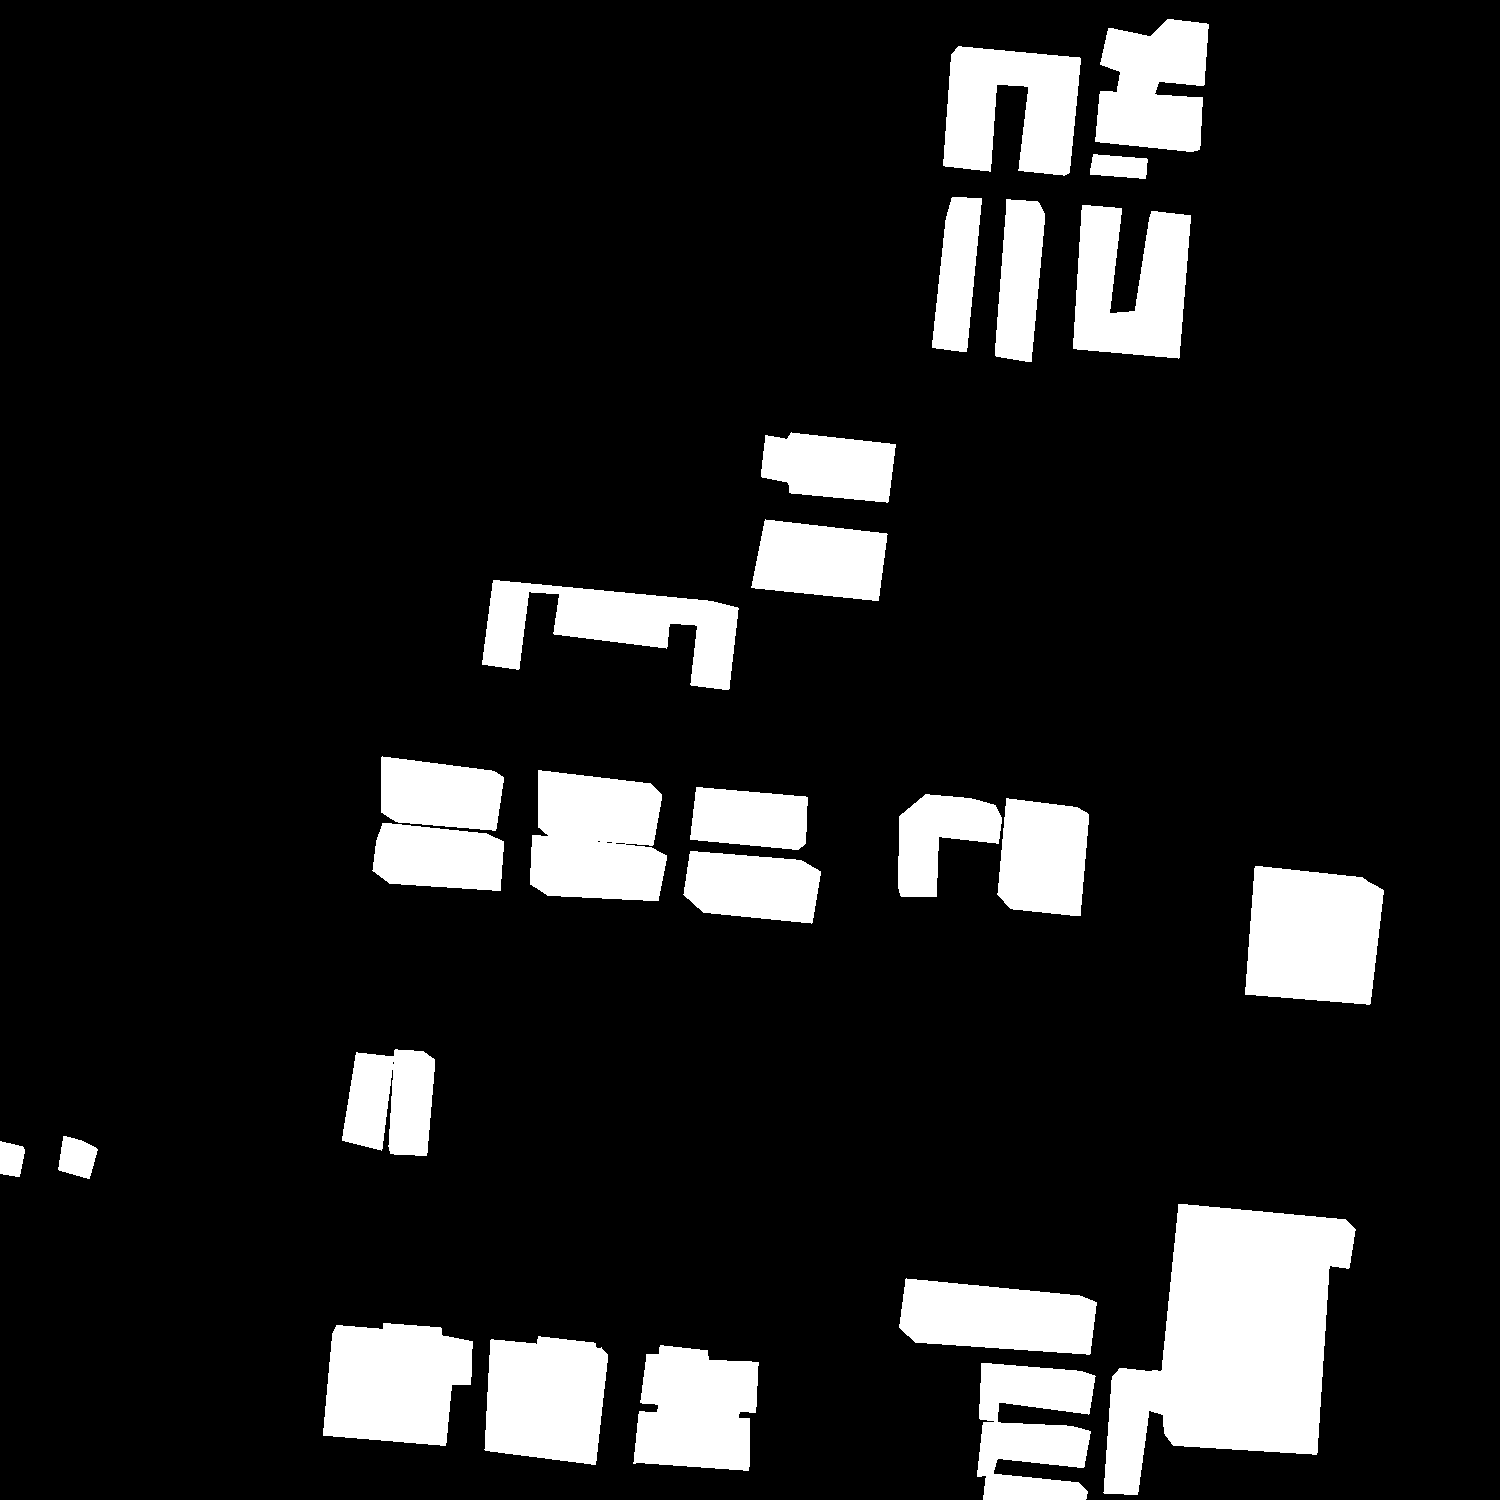
\includegraphics[width=0.7\columnwidth]{rs}
				%Create a subtitle for the figure.
			\caption{Ground truth}
			\label{fig:rt}
		\end{center}
	\end{figure}

% Now we need a bibliography:
%\begin{thebibliography}{5}
%
%	%Each item starts with a \bibitem{reference} command and the details thereafter.
%	\bibitem{HOP96} % Transaction paper
%	J.~Hagenauer, E.~Offer, and L.~Papke. Iterative decoding of binary block
%	and convolutional codes. {\em IEEE Trans. Inform. Theory},
%	vol.~42, no.~2, pp.~429–-445, Mar. 1996.
%
%	\bibitem{MJH06} % Conference paper
%	T.~Mayer, H.~Jenkac, and J.~Hagenauer. Turbo base-station cooperation for intercell interference cancellation. {\em IEEE Int. Conf. Commun. (ICC)}, Istanbul, Turkey, pp.~356--361, June 2006.
%
%	\bibitem{Proakis} % Book
%	J.~G.~Proakis. {\em Digital Communications}. McGraw-Hill Book Co.,
%	New York, USA, 3rd edition, 1995.
%
%	\bibitem{talk} % Web document
%	F.~R.~Kschischang. Giving a talk: Guidelines for the Preparation and Presentation of Technical Seminars.
%	\url{http://www.comm.toronto.edu/frank/guide/guide.pdf}.
%
%	\bibitem{5}
%	IEEE Transactions \LaTeX and Microsoft Word Style Files.
%	\url{http://www.ieee.org/web/publications/authors/transjnl/index.html}
%
%\end{thebibliography}

% Your document ends here!
\end{document}